%%%%%%%%%%%%%%%%%%%%%%%%%%%%%%%%%%%%%%%%%%%%%%%%%%%%%%%
%%%%%%%%%%%%%%%%%%%%%%%%%%%%%%%%%%%%%%%%%%%%%%%%%%%%%%%

\chapter{Inria} \label{INRIA}
\index{Inria}

Anciennement l'acronyme d'``Institut National de Recherche en Informatique et en Automatique'',
Inria, est un \'etablissement public \`a caract\`ere scientifique et technologique (EPST) plac\'e sous la double tutelle du minist\`ere de la
recherche (aujourd'hui \'Education Nationale, Enseignement Sup\'erieur et Recherche) 
et de celui de l'industrie (aujourd'hui \'Economie, Industrie et Num\'erique). 
Il a pour vocation d'entreprendre des recherches fondamentales et appliqu\'ees dans les domaines des
sciences du num\'erique, qui font appel \`a diverses disciplines telles que l'informatique,
l'automatique, les math\'ematiques\footnote{%
Nous vous invitons \`a consulter le texte r\'edig\'e par Philippe Flajolet et G\'erard Huet 
pour mieux comprendre les liens entre math\'ematiques et informatique:
\lien{pauillac.inria.fr/\string~huet/PUBLIC/Mathinfo.doc}.}, 
{\em etc}. Inria est structur\'e
en 8 centres de recherche (CRI) r\'epartis dans plusieurs grandes r\'egions
(Alsace-Lorraine, Aquitaine, Bretagne, Ile-de-France, Nord-Pas-de-Calais, 
Provence-Alpes-C\^ote d'Azur et Rh\^one-Alpes).
Chaque centre de recherche d\'epend de la direction g\'en\'erale et 
est organis\'e de la m\^eme fa\c{c}on~: il est dirig\'e par un directeur ou une directrice d'unit\'e 
dont d\'ependent les services centraux (ressources humaines, service financier, service des
missions, communication, {\em etc.}) et les \'equipes-projets.
Un organigramme de l'institut est pr\'esent\'e sur la page suivante.
Lien officiel : {\lien{www.inria.fr/}}

\section{La politique scientifique}
Tous les quatre ans, Inria se fixe des objectifs prioritaires qui
sont inscrits au ``plan strat\'egique''.

\lien{www.inria.fr/inria/strategie/}

Ainsi, les huit d\'efis scientifiques d'Inria pour les ann\'ees 2013--2017
sont~:
\begin{multicols}{2}
\begin{itemize}
	\item Les syst\`emes ;
	\item Les donn\'ees ;
	\item Les interactions et les usages ;
	\item Les mod\`eles ;
	\item La sant\'e et le bien-\^etre ;
	\item L'\'energie et les ressources naturelles ;
	\item L'environnement et le d\'eveloppement durable ;
	\item La soci\'et\'e et l'\'education.
\end{itemize}
\end{multicols}

Au niveau d'un centre de recherche,
l'instance o\`u s'\'elabore la politique scientifique est le
comit\'e des projets.
Le comit\'e des projets est une instance consultative. Il est en
interaction directe au niveau national avec la commission
d'\'evaluation qui est charg\'ee de proc\'eder \`a l'\'evaluation
des \'equipes de recherche et des personnels scientifiques. Le
comit\'e des projets est charg\'e du suivi des affaires
scientifiques du CRI~: activit\'es scientifiques, examen des demandes
de cr\'eation ou d'arr\^et des \'equipes-projets,
{\em etc.} Il a \'egalement pour r\^ole l'\'echange et la diffusion
d'informations concernant les activit\'es scientifiques des
\'equipes-projets.

La commission d'\'evaluation, quant \`a elle, pr\'epare
les travaux du conseil scientifique en contribuant notamment \`a
d\'efinir les orientations des activit\'es de l'institut. En effet,
le conseil scientifique est l'instance de r\'eflexion et de
proposition de l'institut en mati\`ere de politique scientifique. Il
donne son avis au conseil d'administration sur les grandes
orientations de la politique scientifique de l'institut, les
programmes de recherche et le rapport annuel d'activit\'e~:
\lien{www.inria.fr/rapportsactivite}.

\begin{center}
\liens{www.inria.fr/institut/organisation/organigramme-general}
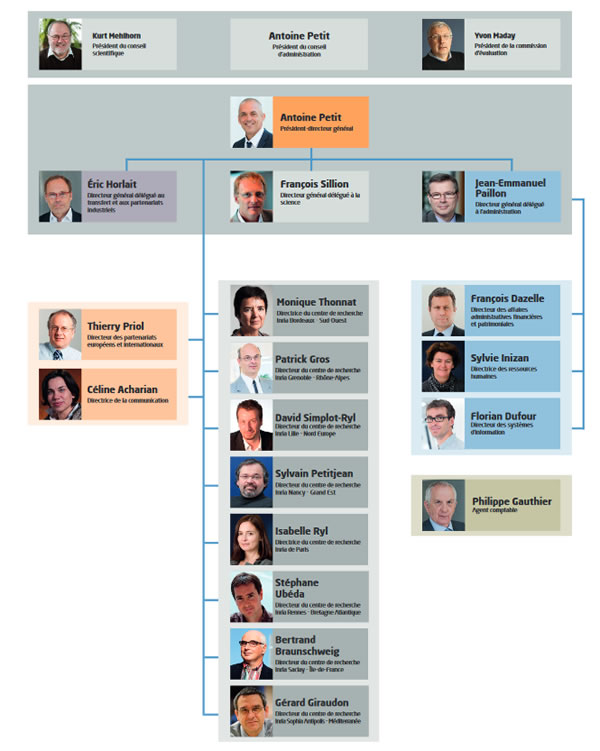
\includegraphics[width=11cm]{Images/organigramme-inria-2016.jpg}
\end{center}

\section{Quelques chiffres}

Le budget primitif d'Inria pour l'ann\'ee 2015 est de
230\,M\euro{}, dont 27\,\% de ressources propres (contrats de recherche
et produits de valorisation). Sur les 4400 personnes (approximativement) pr\'esentes aujourd'hui \`a
Inria, environ 60\% sont des personnels Inria. 
Parmi les titulaires, un tiers sont des chercheurs
et deux tiers des ing\'enieurs, techniciens et administratifs. 

R\'epartis au sein d'environ 230 \'equipes-projets, 
plus de 3400 scientifiques, toutes disciplines confondues,
travaillent \`a l'institut, 
dont environ 1400 chercheur$\cdot$ses et enseignant$\cdot$es-chercheur$\cdot$ses, 
1300 doctorant$\cdot$es et 800 contractuel$\cdot$les
(post-doctorant$\cdot$es, ing\'enieur$\cdot$es expert$\cdot$es et ing\'enieur$\cdot$es associ\'e$\cdot$es).

\liens{panorama.inria.fr/chiffres-cles/}

\section{Les \'equipes-projets de recherche}
\label{sec. projets INRIA}
\index{Equipes-projets Inria (EPI)}

Les \'equipes-projet Inria (EPI) r\'eunissent, autour d'une personnalit\'e scientifique, un groupe de chercheur$\cdot$ses, d'enseignant$\cdot$es chercheur$\cdot$ses, de doctorant$\cdot$es et d'ing\'enieur$\cdot$es. Elles ont toutes un objectif commun : relever un d\'efi scientifique et technologique dans l'un des domaines de recherche prioritaires de l'institut d\'efinis dans le plan strat\'egique.


Pour obtenir le label ``EPI'', le projet de l'\'equipe de recherche doit \^etre approuv\'e par une commission d'\'evaluation comp\'etente dans son domaine scientifique. Une fois labellis\'ee, l'EPI a quatre ans pour mener \`a bien son programme de recherche et atteindre ses objectifs. Pour ce faire, elle dispose de ressources propres. Au terme de quatre ann\'ees, l'EPI fait \`a nouveau l'objet d'une \'evaluation scientifique. Elle peut ainsi \^etre prorog\'ee ou bien arr\^et\'ee. Reconduite deux fois tout au plus, l'EPI a une dur\'ee maximale de vie de 12 ans et une dur\'ee moyenne de 8 ans.

\subsection*{L'\'evaluation des \'equipes-projets}
\index{Evaluation ! \`a l'INRIA}

Toutes les \'equipes-projets d'un m\^eme \textsl{th\`eme} sont
\'evalu\'ees simultan\'ement, de mani\`ere \`a rendre possible les
comparaisons, et \`a permettre de d\'egager une vision globale de la
politique d'Inria sur ce th\`eme. Un groupe d'une dizaine
d'expert$\cdot$es ext\'erieur$\cdot$es, issu$\cdot$es de la communaut\'e scientifique et de
l'industrie, examine les rapports d'activit\'e et les publications
\'emanant des EPI concern\'ees, ainsi que des documents d\'ecrivant
la politique d'Inria et les crit\`eres d'\'evaluation propos\'es.
Depuis 2002, cette \'evaluation se d\'eroule en anglais, ce qui a
permis d'\'elargir consid\'erablement le bassin d'\'evaluateurs
potentiels. Le rapport, qui est r\'edig\'e sans la moindre
interf\'erence de la direction d'Inria, comporte \`a la fois une
analyse globale du th\`eme et des recommandations d\'etaill\'ees
concernant chaque EPI.

Les chefs d'\'equipes-projets r\'edigent ensuite des r\'eponses qui sont
examin\'ees en comit\'e des projets, puis au niveau de la commission
d'\'evaluation. La commission d'\'evaluation r\'edige \`a son tour
des recommandations au$\cdot$\`a la Pr\'esident$\cdot$e d'Inria qui consulte le
conseil scientifique. Le rapport d'\'evaluation externe et l'avis
du conseil scientifique ont en fait un impact durable sur la
strat\'egie de l'institut.

\`A l'issue de tout ce processus, une d\'ecision formelle est sign\'ee
par la ou le Pr\'esident$\cdot$e Directeur$\cdot$trice G\'en\'eral$\cdot$e qui autorise la poursuite
de l'\'equipe-projet, ou demande son arr\^et. Lorsqu'une EPI s'arr\^ete, les
chercheuses et chercheurs ont le temps de r\'efl\'echir pour savoir s'ils
souhaitent rejoindre une autre EPI, ou proposer de nouveaux
objectifs pour cr\'eer une nouvelle EPI, en suivant les conseils du
directeur de l'unit\'e et du pr\'esident du comit\'e des projets.

\section{La commission d'\'evaluation}
\index{Commission d'\'evaluation INRIA}
\index{Evaluation ! \`a l'INRIA}

La commission d'\'evaluation d'Inria, dot\'ee d'une forte autonomie, est au c{\oe}ur de l'\'evaluation scientifique de l'Institut. Elle est compos\'ee de personnalit\'es scientifiques \'elues et nomm\'ees d'Inria et d'expert$\cdot$es ext\'erieur$\cdot$es \`a l'Institut. En liaison avec la Direction des recherches, elle coordonne l'\'evaluation externe du travail des \'equipes-projets Inria, domaine de recherche par domaine de recherche. Elle forme le c\oe ur des jurys d'admissibilit\'e des concours qui contiennent aussi des personnalit\'es ext\'erieures nomm\'ees par la Direction g\'en\'erale, ainsi que les commissions proposant les promotions internes. Elle intervient enfin dans l'\'evaluation de la cr\'eation des projets et dans celle des actions scientifiques collectives d'Inria.

Dans le cadre de ses missions, la commission d'\'evaluation constitue des groupes de travail sur des sujets li\'es \`a l'\'evaluation (exemples : parit\'e homme-femme, \'evaluation des logiciels, du transfert technologique, de la diffusion scientifique, {\it etc}). Elle m\`ene \'egalement des r\'eflexions de nature strat\'egique sur l'\'evolution des domaines scientifiques d'Inria et l'\'evolution associ\'ee du m\'etier de chercheur.

La commission d'\'evaluation compte 40 membres au total :
\begin{itemize}
\item 20 membres nomm\'es par le$\cdot$la pr\'esident$\cdot$e de l'institut dont 10 sur proposition du ou de la pr\'esident$\cdot$e du conseil scientifique~;
\item 20 membres \'elus par et parmi le personnel de l'\'etablissement, selon des modalit\'es fix\'ees
par d\'ecision de la ou du pr\'esident$\cdot$e de l'institut.
\end{itemize}
Les membres nomm\'es sont choisis, pour la moiti\'e d'entre eux, parmi les personnalit\'es scientifiques
ext\'erieures \`a l'institut. Le$\cdot$La pr\'esident$\cdot$e de cette commission est d\'esign\'e$\cdot$e parmi ses membres par le$\cdot$la
 pr\'esident$\cdot$e de l'institut, sur proposition du$\cdot$de la pr\'esident$\cdot$e du conseil scientifique.  
 
\liens{www.inria.fr/institut/organisation/instances/commission-d-evaluation}
